\chapter{Data and Research Design}
\label{data}

To measure the welfare effects of individualizing life-cycles compared to default life-cycles we will construct the stock, housing and labor income series from the past data, define the expected rates of return, volatilities and correlations from conventions and simulate a 30-year investment timespan for every type of investor until the retirement. We will then calculate certainty equivalent consumption levels and compare them. 

\section{Data}

\subsection{Stocks}
To measure the stock series we used BIST 30 index which measures the aggregate performance of 30 best companies in Turkey. The monthly data is taken from Borsa Istanbul. We can see from Figure 4.1 the general upward trend with collapse during 2008 crisis.

\begin{figure}
	\centering
    \begin{minipage}{0.45\textwidth}
		\centering
		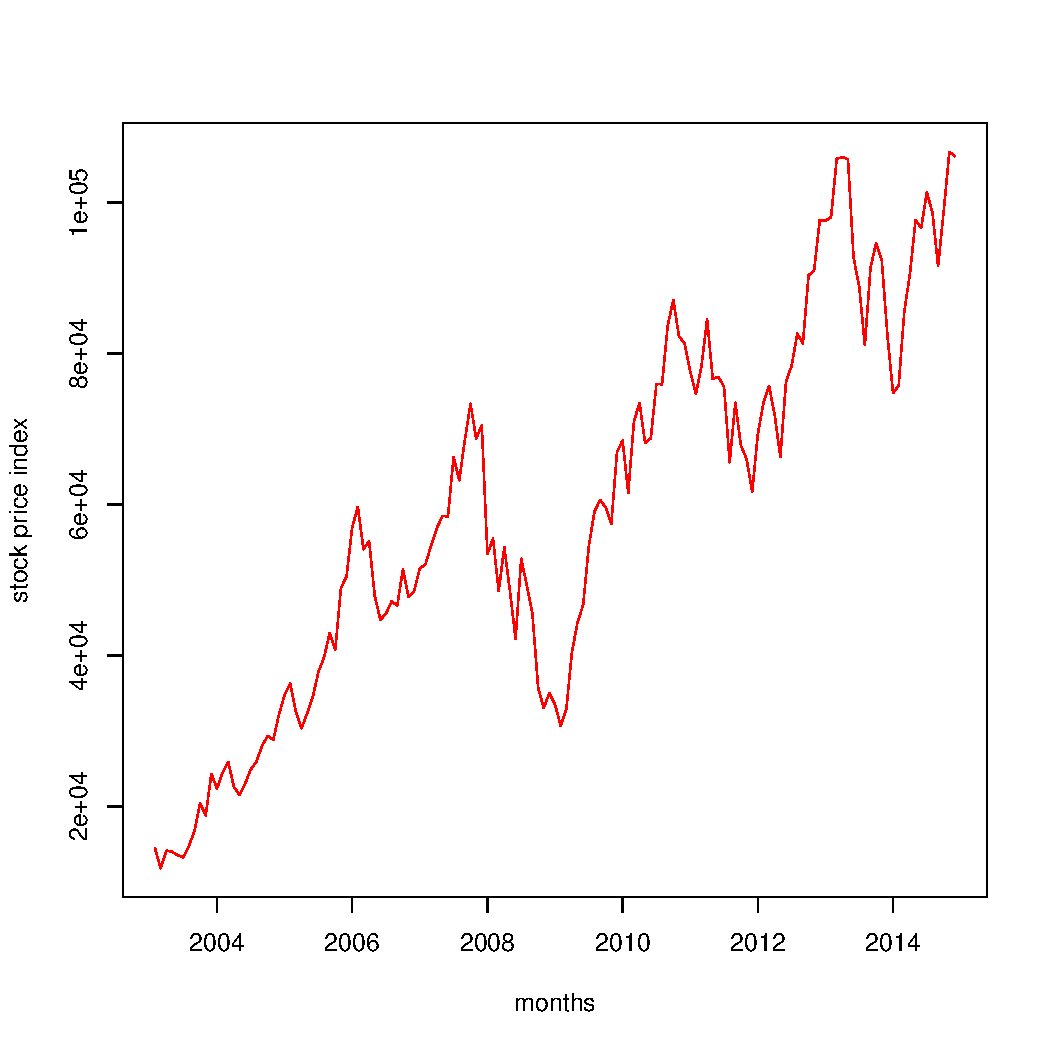
\includegraphics[scale=0.4]{figs/bist.pdf}
		\caption{BIST30 Turkish stock market performance index}
	\end{minipage}
	\hfill
    \begin{minipage}{0.45\textwidth}
		\centering
		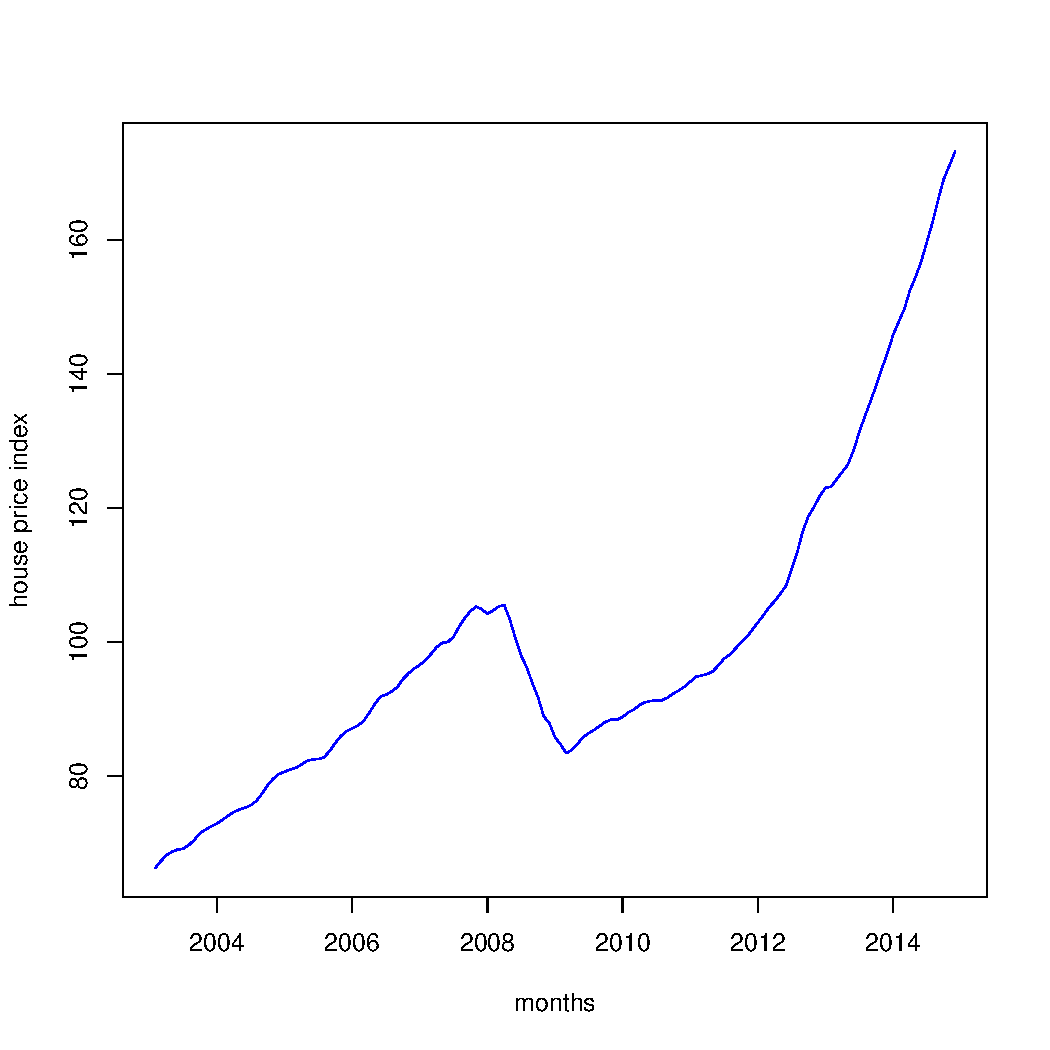
\includegraphics[scale=0.4]{figs/reidin.pdf}
		\caption{REIDIN Turkish House Price Index}
	\end{minipage}
\end{figure}

\subsection{Housing}
To measure the house prices we used Reidin data on Istanbul house prices. AEINDEXF Figure 4.2


\subsection{Labor income}
We used TUIK's Household Budget Survey Data and regression results of Aktug, Kuzubas, Torul (2017). We have 55 thousand panel data points for 170 households for 2001 to 2014 years. We can observe the hump-shaped lifetime income distribution in Figure 4.3. This corresponds well to an established literature in this field.

\begin{figure}[h]
	\centering
	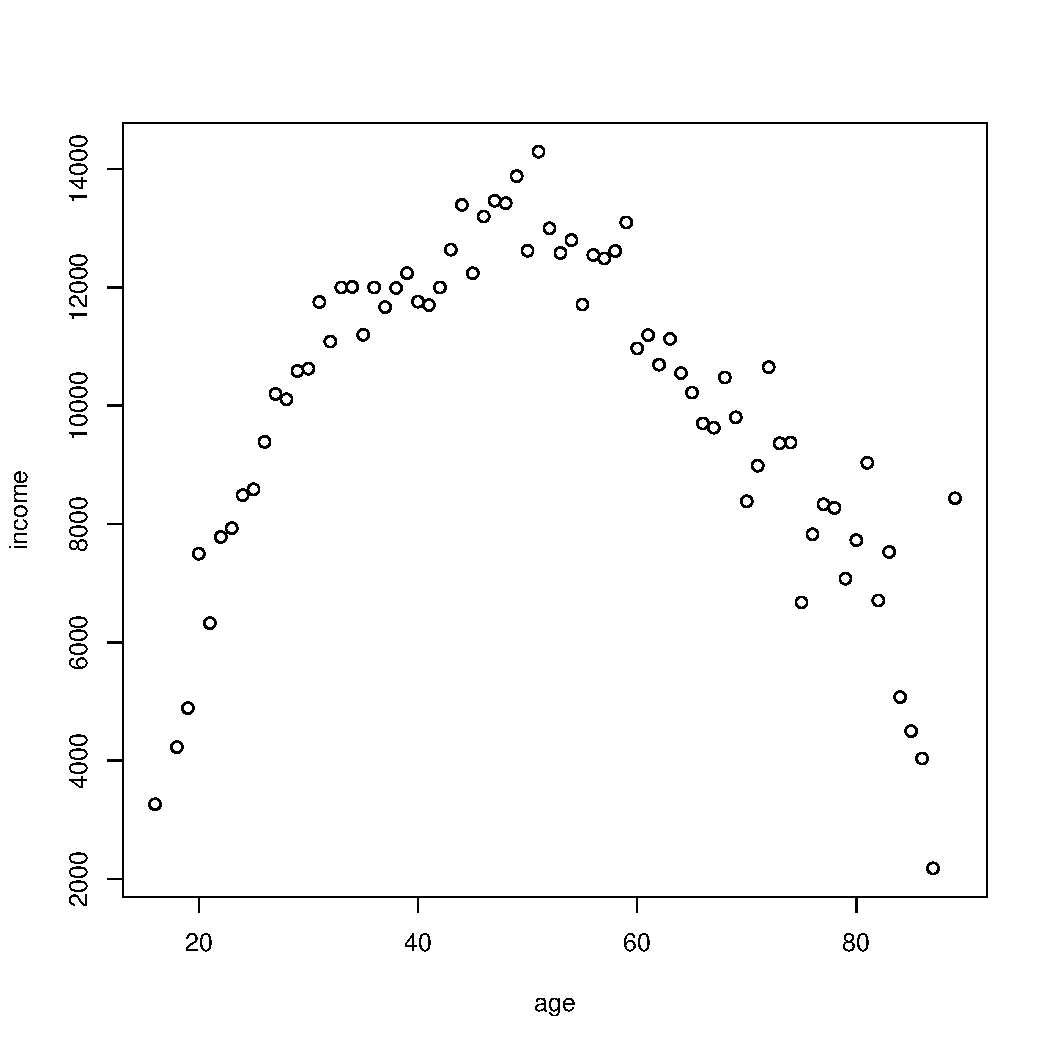
\includegraphics[scale=0.5]{figs/wage2median.pdf}
	\caption{Median Turkish salaries by age}
\end{figure}

\section{Research Design}
In our simulation we will compare welfare effects of default lifecycles and individualized lifecycles defined below. Default lifecycles are taken from the ones mentioned in our literature review chapter (100-age etc.) and from the real investment strategies of the largest Turkish pension fund provider. Individualized lifecycles will be calculated using Munk's optimal portfolio formula from previous chapter. In the same manner as Olear(2014) we will use wage growth rate, stock-income correlation and idiosyncratic labor income risk to model heterogeneity in education, sector and SOMETHING HERE respectively.

\subsection{Default Lifecycles}
100-age\\
200-2.5age\\
AHL: agresif: 50\% 50\% \\
AH0: orta riskli: 30\% \\

\subsection{Individualized Lifecycles}
Let's now consider the heterogeneities one at a time:

\subsubsection{Heterogeneity in education}
In line with Olear's (2016) approach we model the heterogeneity in education using the differences in wage growth rates. Indeed, we expect the salaries for higher education level to grow faster than for the lower education level. Some of this expectation comes from the fact that people with lower education are restricted in their career ladders and cannot rise very high in a workplace. Another intuition is that while college dropouts start working immediately, college graduates and graduate students continue to study and thus report zero income. When they graduate, their salary immediately rises from zero to the average salary, and this constitutes a steeper wage growth curve at the beginning of their lives. Figure 4.4 shows the wage series for different levels of education. Note that the curves for the lowest education levels are practically flat and the those for the highest education levels have varying non-zero slopes. 

\begin{figure}[h]
	\centering
	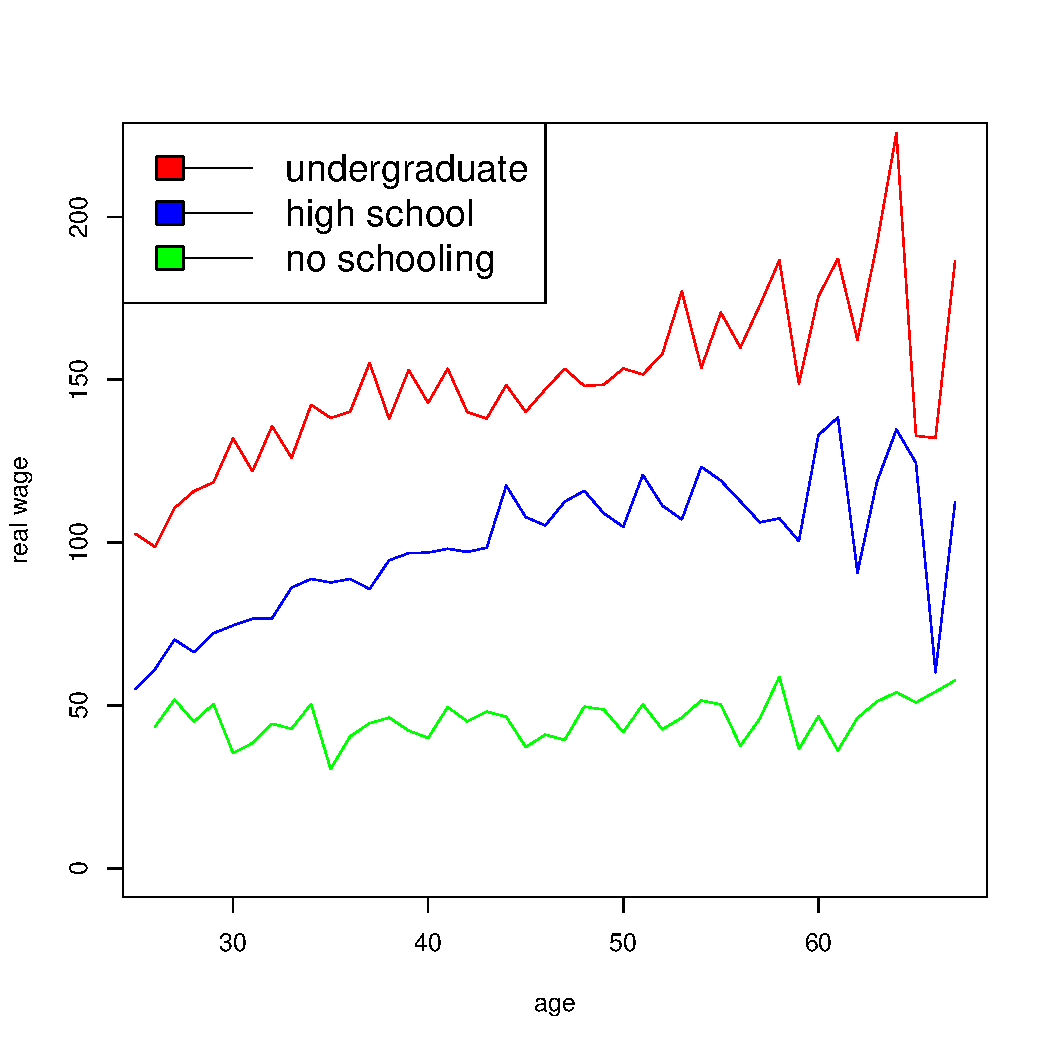
\includegraphics[scale=0.6]{figs/wage2educ.pdf}
	\caption{Lifetime wage dynamics by education level}
\end{figure}

Performing kinked regressions of log wages on ages yielded best linear fits for three different education levels of our choice: postgraduate, high school, and no schooling. The corresponding labor income growth rates can be characterized as steep, moderate, and flat respectively. We considered wage data until 60 years, as Turkish retirement age is at 57, and have added empirically best kinks at ages 35 and 45. The results are summarized in Table 4.1 and illustrated in Figure 4.5. In this figure red lines represent the actual wages dynamics for postgraduate, high school, and no schooling, and blue lines are plots of the percentage changes proposed in Table 4.1, where the starting points all correspond to the actual starting points from the data. Figure 4.6 illustrates the same parameterized curves without actual wage curves. 

\begin{table}
	\centering
	\begin{tabular}[c]{l|ccc}
		Age&Flat&Moderate&Steep\\
		\hline
		0-35&0\%&3.5\%&6.5\%\\
		36-45&0\%&3\%&2\%\\
		46-60&0\%&0\%&0\%\\
	\end{tabular}
	\caption{Estimated benchmark wage growth rates}
\end{table}


\begin{figure}[h]
	\centering
    \begin{minipage}{0.45\textwidth}
		\centering
		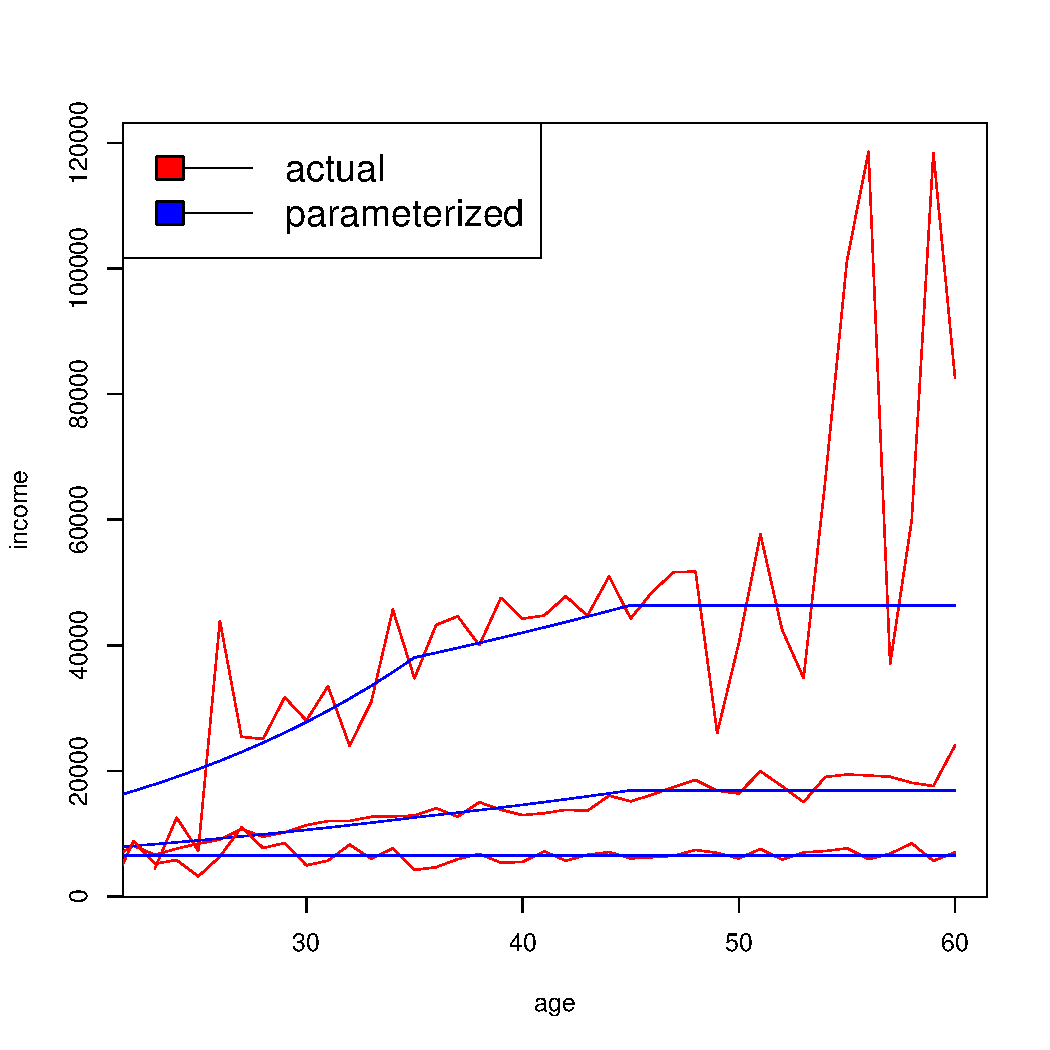
\includegraphics[scale=0.4]{figs/heterwage.pdf}
		\caption{Actual and parameterized benchmark wage dynamics by age}
	\end{minipage}
	\hfill
    \begin{minipage}{0.45\textwidth}
		\centering
		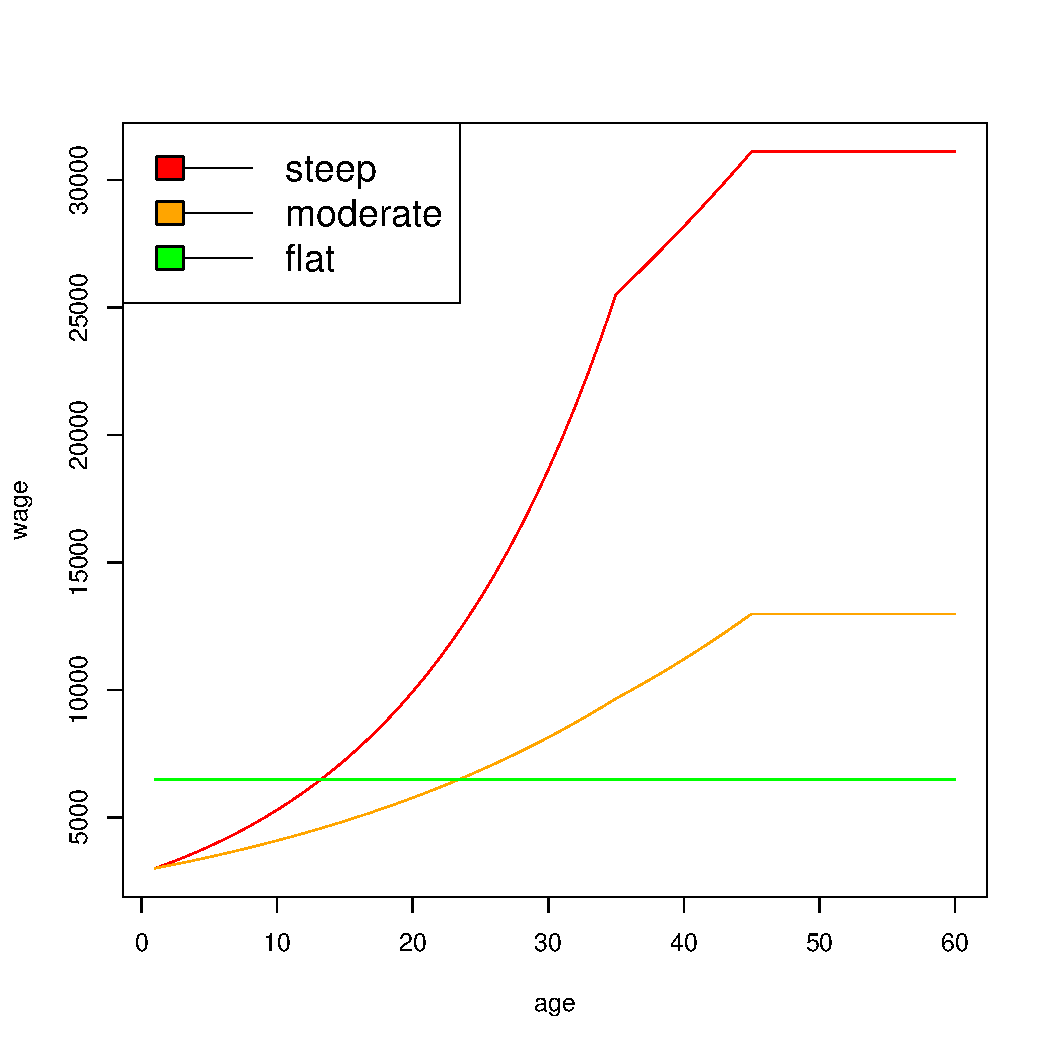
\includegraphics[scale=0.4]{figs/heterwageless.pdf}
		\caption{Parameterized wage dynamics by age}
	\end{minipage}

\end{figure}


\subsubsection{Heterogeneity in sectors}




\subsection{Parameters}
In our simulation we use the conventional parameters for risk aversion, retirement age, initial income. We also use Sermaye Piyasalari Kurulu (SPK)'s forward-looking parameters for expected returns and volatilities of house, stock, and labor returns. As summarized in table 4.1. 


The data on survival probability for all ages is taken from TUIK (Turkish Statistical Institute)'s database.  

\begin{table}
	\centering
	\begin{tabular}[c]{lll}
		Parameter&Description&Value\\
		\hline
		1&1&1\\
		1&1&1\\
		1&1&1\\
		1&1&1\\
		1&1&1
	\end{tabular}
	\caption{Hello}
\end{table}
